%
% File acl2017.tex
%
%% Based on the style files for ACL-2015, with some improvements
%%  taken from the NAACL-2016 style
%% Based on the style files for ACL-2014, which were, in turn,
%% based on ACL-2013, ACL-2012, ACL-2011, ACL-2010, ACL-IJCNLP-2009,
%% EACL-2009, IJCNLP-2008...
%% Based on the style files for EACL 2006 by 
%%e.agirre@ehu.es or Sergi.Balari@uab.es
%% and that of ACL 08 by Joakim Nivre and Noah Smith

\documentclass[11pt,a4paper]{article}
\usepackage[hyperref]{acl2017}
\usepackage{times}
\usepackage{latexsym}
\usepackage{bm}
\usepackage{graphicx}
\usepackage{amsmath}
\DeclareMathOperator*{\argmax}{argmax} % thin space, limits underneath in displays
\usepackage{url}

\usepackage{tabularx,booktabs}
\newcolumntype{C}{>{\centering\arraybackslash\hsize=.5\hsize}X} % centered version of "X" type
\setlength{\extrarowheight}{1pt}


\usepackage{adjustbox}
\usepackage{float}





\aclfinalcopy % Uncomment this line for the final submission
%\def\aclpaperid{***} %  Enter the acl Paper ID here

%\setlength\titlebox{5cm}
% You can expand the titlebox if you need extra space
% to show all the authors. Please do not make the titlebox
% smaller than 5cm (the original size); we will check this
% in the camera-ready version and ask you to change it back.

\newcommand\BibTeX{B{\sc ib}\TeX}

\title{CS395T: Shift-Reduce Parsing Project Report}

\author{Zeyuan Hu \\
  Computer Science Department \\
  University of Texas at Austin \\
  Austin, Texas \\
  {\tt iamzeyuanhu@utexas.edu} \\
}

\date{}

\begin{document}
\maketitle

\begin{abstract}
In this project, I implement a purely greedy parser using a logistic regression classifier
to generate shift-reduce decisions. Then, I implement a global beam-search parser that
searches over the same space but perform the inference over the whole sentence. Lastly, 
I tried to implement the arc eager transition system and I will talk about some 
questions raided during the arc-eager system implementation. 
\end{abstract}

\section{Collaborators}
Zhan Shi, Danlu Wang

\section{Introduction}

Dependency parsing is a task about assigning syntactic annotations for a given sentence.
Specifically, the task is to predict the syntactic parents and dependency labels and thus form
a dependency tree. For example, in a sentence \emph{education ads:}, the task will predict the 
parent of word \emph{education} is \emph{ads}. Systems for dependency parsing
either operate in a graph-based or trainsition-based paradigm. In this project,
we explore the transition-based systems with the greedy and the global beam-search
parsers, which make local decisions and process the dependency tree incrementally
from left-to-right. There are four components in both systems: input buffer, stack, oracle, and
dependency relations. The parser's \emph{state} is captured by a \emph{stack} of partial
dependency trees and a \emph{buffer} of words waiting to be processed. During the parsing,
we consult \emph{oracle} to get the decisions on how to process the dependency trees and words.
Then, we apply decisions and get \emph{dependency relations}. In this project, we construct 
our greedy parser oracle using a logisitic regression classifier and our global beam-search parser
oracle using Structured SVM (SSVM). 

\section{Implementation Details}

\subsection{Greedy Parser}

For the greedy parser, we first build a \verb|feature_cache| by walking through the gold states of
each sentence and then apply all three possible actions to those states. The data structure
for the \verb|feature_cache| is a list of \verb|feature_matrix| with dimension $3$ by $23$, with
$3$ representing all three possible actions and $23$ representing the number of features.
Then, for each epoch, I calculate the $P(y|x)$ for all possible $y$, which, in this case, are
all three possible actions. Once we calculate $P(y|x)$, we can get the gradient
$f_i(x_j,y_j^*) - \sum_y f_i(x_j,y)P(y|x_j)$ with $f_i(x_j,y_j^*)$ representing the indicator
function of a gold feature value. This translates into the program by incrementing the weights
associated with the gold features by one. The gradients are stored in a $3$ by $23$ matrix
with each row corresponding to the gradients of the weights associated with each possible
action. Once we have the gradients, we can perform the stochastic gradient descent (SGD) update
to the weights. After the training phase, we build the oracle by caclulating $\argmax_yP(y|x)$.

\subsection{Global Beam-Search Parser}

The global beam-search parser has the same code structure as the greedy parser. We first train
the model to get the weights and then we construct the parser using those weights. One assumption
made by the greedy parser is that the oracle will give the correct operator at each step of the
parse, which is unlikely to be true \cite{Jurafsky:2017}. In order to handle this issue, we need
to take a look at alternative choices at each step, which leads to the beam search of all the possible
parse sequences. Like the greedy parser, we first implement a \verb|feature_cache| to facilitate our
access to the features and help us to initialize our \verb|feature_weights|. In each epoch, for each
sentence, we initialize our beam with action "S" because of 
the specification of arc-standard transition system. Then, for all the following beams, we need to check
whether we are already in the final state. If not, we apply all three actions to the states sit in the beam
and push the newly-created states onto the current beam. Afterwards, we use the early updating strategy
by performing the SSVM update if we find the gold actions already fall out of the beam. If that is not the case,
we perform the SSVM update using the features that are cumulative over the whole sentence.

\subsection{Arc Eager Transition System}

So far, we have assumed that the transitions between states follow the arc standard system. As the extension
to the project, I want to explore the alternative transition system: arc eager. Unfortunately, I meet some
issues during the implementations. The major one comes from the inconsistent
definition of the precondtion for each action under in the system. We can apply \verb|LeftArc| action as long as the top
of the stack is not the root node. For \verb|Shift| action, we can apply it as long as there are tokens inside the buffer.
There is no restriction for the \verb|RightArc|. However, for \verb|Reduce| operation, there are
discrepancies from different literature. Jurafsky~\shortcite{Jurafsky:2017} does not explicitly talk about this issue
but from Figure 14.10 example, it seems like \verb|Reduce| can only happen when there is no tokens in the buffer and
there are elements left on the stack other than root. This conjecture is confirmed by Goldberg and Nivre~\shortcite{GoldbergN12},
which in the paper, they state that "The REDUCE transition pops the stack and is subject to the preconditions that the top
token has a head". However, some literature thinks that the precondition should also include: the top of the stack has all its
children attached to it \cite{cmuarc}. During the implementation, I find that there might be some exceptions to the rules. For example, 
the sentence \emph{Influential members of the House Ways and Means Committee introduced legislation that would restrict
how the new savings-and-loan bailout agency can raise capital, creating another potential obstacle to the government's sale of sick
thrifts.} has a state: \verb|[-1, 1, 2, 5, 9, 10, 13, 21, 24, 27]| for the stack,
\verb|[36]| for the buffer, and \verb|{0: 1, 2: 1, 4: 5, 5: 2, 6: 5, 7: 8, 8: 5,|
\verb|10: 9, 12: 13, 13: 10, 18: 19, 19: 21,| 
\verb|20: 21, 21: 13, 22: 21, 26: 27, 27: 24,|
\verb|28: 27, 29: 30, 30: 32, 31: 30, 32: 28,|
\verb|33: 32, 34: 35, 35: 33}| for the dependency relations. 
Since there is no parent-child relation between \verb|27| and \verb|36| and we cannot apply \verb|Reduce|
as well, the only option left is \verb|Shift|. However, if we check carefully for the elements on the stack, we find that
\verb|36|'s parent is \verb|24|, \verb|24|'s parent is \verb|13|, \verb|13|'s parent is \verb|10|, \verb|10|'s parent is \verb|9|, and 
\verb|9|'s parent is \verb|-1|, which are all on the stack. Since there is no operation allowing us to examine two elements on the stack in 
the arc eager system, the only choice we left is 
\verb|Reduce|, which will lead to the failure of parsing. The detailed code implementation and reproduction can be found under the directory
\verb|hw2-arc-eager|.


\section{Experiments}

Figure 1 shows the result of the UAS score for both the greedy parser and the
the global beam-search parser on the development set. Table 1 shows the parameters
experimentation with different optimizer, learning rate, epoches, sentences and batch
size for different parsers. In general, as the number of epoches in the training phase increases, 
the UAS scores increase. The number of training examples (i.e., sentences) play a major role
in the parsing result. The target UAS scores (i.e., $78$ for greedy parser and $75$ for global beam-search parser)
can only be achieved by using the whole training examples (i.e., $39832$ sentences).

\begin{figure}[h]
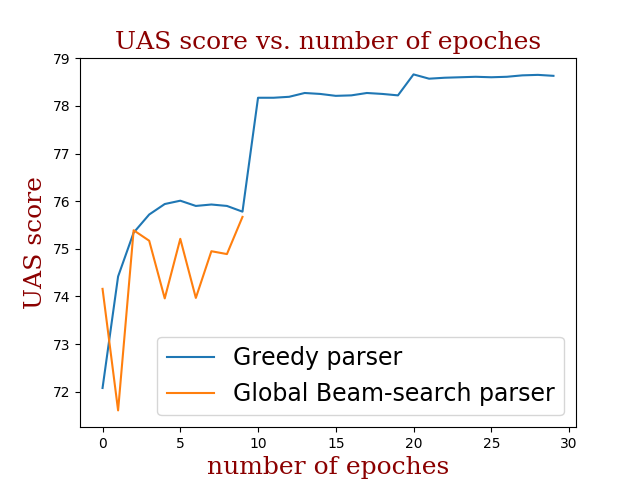
\includegraphics[scale=0.5]{uas.png}
\caption{UAS score vs. number of epoches in development set}
\end{figure}

\begin{table*}
\caption{Impact of the parameters on the UAS score}
\label{data-table}
\begin{tabularx}{\textwidth}{@{}l*{8}{C}c@{}}
\toprule
Parser    & Optimizer & Learning Rate & Epoches & Sentences     & Batch Size     & UAS    \\    
\midrule
Greedy    & SGD        & 0.2              & 10         & 5000          & 1         & 72.27  \\    
Greedy    & SGD        & 0.2            & 20      & 5000           & 1                & 74.67  \\   
Greedy    & SGD       & 0.2             & 30        & 5000          & 1               & 75.81  \\   
Greedy    & SGD       & 0.2              & 40         & 5000         & 1               & 75.74  \\   
\addlinespace
Greedy    & SGD       & 0.2              & 30         & 6000          & 1              & 76.35  \\   
Greedy    & SGD       & 0.2              & 30      & 7000         & 1               & 76.43  \\  
Greedy    & SGD       & 0.2              & 30      & 39832          & 1                & \textbf{78.60}  \\    
Global    & Adagrad(0.0001, 5) & 5    & 10      & 39832          & 20               & \textbf{75.67}  \\ 
\bottomrule
\end{tabularx}
\end{table*} 


\section{Conclusion and Future Work}

In this project, I implement the greedy parser and the global beam-search parser.
I show the importance of the training data to the system performance. I also tried to 
implement arc eager transition system as extension but there are some questions raised during
the implementation. In the future, I can finish the implementation of arc eager transition system 
and perform feature engineering to improve the performance of both parsers.

\bibliography{acl2017}
\bibliographystyle{acl_natbib}

\end{document}
